\documentclass[UTF8,a4paper,12pt]{ctexart}
\usepackage[margin=2.5cm]{geometry}
\usepackage{setspace}
\usepackage{amsmath,amssymb}
\usepackage{booktabs}
\usepackage{longtable}
\usepackage{array}
\usepackage{tabularx}
\usepackage{graphicx}
\usepackage{float}
\usepackage{caption}
\usepackage{enumitem}
\usepackage{xcolor}
\usepackage{hyperref}
\usepackage{tikz}
\usetikzlibrary{arrows.meta,positioning,shapes.geometric,fit,calc}

\linespread{1.35}
\setlength{\parskip}{0.45em}
\setlength{\parindent}{2em}
\setlist[itemize]{leftmargin=2em}
\setlist[enumerate]{leftmargin=2.2em}

\hypersetup{
  colorlinks=true,
  linkcolor=black,
  urlcolor=blue
}

\definecolor{boxblue}{RGB}{232,242,252}
\definecolor{boxgreen}{RGB}{232,248,238}
\definecolor{boxorange}{RGB}{253,243,227}
\definecolor{boxgray}{RGB}{244,244,244}

\tikzset{
  nodebox/.style={
    rectangle,
    rounded corners=2pt,
    draw=black!55,
    thick,
    minimum width=2.5cm,
    minimum height=0.95cm,
    align=center,
    font=\small,
    fill=boxblue
  },
  nodebox2/.style={
    rectangle,
    rounded corners=2pt,
    draw=black!55,
    thick,
    minimum width=2.5cm,
    minimum height=0.95cm,
    align=center,
    font=\small,
    fill=boxgreen
  },
  nodebox3/.style={
    rectangle,
    rounded corners=2pt,
    draw=black!55,
    thick,
    minimum width=2.5cm,
    minimum height=0.95cm,
    align=center,
    font=\small,
    fill=boxorange
  },
  decision/.style={
    diamond,
    aspect=1.8,
    draw=black!60,
    thick,
    align=center,
    font=\small,
    fill=boxgray,
    inner sep=1pt
  },
  flow/.style={-{Stealth[length=3mm]}, thick, black!70}
}

\title{\heiti 开题报告自学讲义\\[0.4em]
\Large 面向复杂金融查询的检索增强问答系统\\
\large （由浅入深·纯中文·工程对齐版）}
\author{基于开题报告与仓库 SEAL 结果整理}
\date{2026年3月12日}

\begin{document}
\maketitle
\thispagestyle{empty}

\begin{center}
\begin{minipage}{0.92\textwidth}
\small
\textbf{使用说明}：本讲义对应文件与证据源为
\texttt{报告/开题报告\_石延斌\_U202216405\_题目\_2026年3月11日.pdf}、
\texttt{docs/TABLE\_MAIN.md}、
\texttt{docs/TABLE\_NUMERIC.md}、
\texttt{docs/MILESTONE\_REPORT.md}、
\texttt{thesis/figures\_seal/ThemeA/figures/*}。
讲义目标不是“堆概念”，而是帮你从零基础一步步理解：问题为什么难、方法怎么搭、实验说明了什么、目前哪里还没闭环。
\end{minipage}
\end{center}

\newpage
\tableofcontents
\newpage

\section{问题背景}
\subsection{先讲直觉}
你这项研究要解决的是一个很真实的问题：面对很长的金融披露文件（例如年报），人很难在短时间内又快又准地找到证据并回答问题。
金融问题常常不是“一个句子对应一个答案”，而是同时要求系统做到三件事：先找到证据，再对齐年份，最后给出可核验的数值或结论。
如果只靠大模型直接“生成”，容易出现看起来流畅但无法核对的答案。

\subsection{再讲定义}
\textbf{复杂金融查询}可以简单理解为：在一个问题里同时有专业术语、时间约束和数值要求。  
\textbf{检索增强问答}可以理解为：先去文档里找证据，再根据证据作答，而不是只凭模型参数记忆回答。

\subsection{再讲本报告中的实现与结果}
你的开题报告明确把目标聚焦在三个核心能力上：证据定位、年份对齐、数值可靠性。
对应仓库工程，当前已经形成可冻结的实验链路（SEAL）：
\begin{itemize}
  \item matrix\_id：\texttt{20260228\_055920\_06d6bb}
  \item 20 个实验 run 全部 \texttt{status=ok}
  \item 主结果表、数值表、消融表已更新
\end{itemize}
这说明当前讲义可以建立在\textbf{稳定证据}上，而不是停留在“想法阶段”。

\subsection{易错点}
\begin{itemize}
  \item 把“问题复杂”理解成“问题很长”。实际上短问题也可能很复杂（例如缩写+年份+同比）。
  \item 把“模型会回答”理解成“答案可靠”。金融场景里，可靠性必须可追溯到证据。
  \item 把“实验跑通”理解成“结论成立”。跑通是必要条件，稳定增益才是结论条件。
\end{itemize}

\subsection{自测题}
\begin{enumerate}
  \item 为什么金融问答必须强调“证据可核验”，而不仅是“语言通顺”？
  \item 同一个短问题为什么也可能是复杂查询？
  \item 你的项目里“可冻结”具体意味着什么？
\end{enumerate}

\section{核心概念}
\subsection{先讲直觉}
先把全局地图建立起来：你做的不是单模型调参，而是一条系统链路。
链路中每个模块有输入、有输出、有开关，因此可以做干净的对照实验。

\subsection{再讲定义}
\begin{itemize}
  \item \textbf{稀疏检索（BM25）}：依赖关键词匹配，擅长精确字符串命中。
  \item \textbf{稠密检索（Dense）}：把查询和文本映射到向量空间，擅长语义匹配。
  \item \textbf{混合检索（Hybrid）}：融合前两者分数，兼顾关键词与语义。
  \item \textbf{查询扩展（PQE）}：在查询中补充关键线索（尤其是年份线索）提高召回。
  \item \textbf{门控计算（Calculator Gating）}：只有条件满足才计算，否则回退。
\end{itemize}

\subsection{再讲本报告中的实现与结果}
根据里程碑文档，当前链路可抽象为：
查询 $\rightarrow$ 检索模式选择 $\rightarrow$（可选）扩展/多步检索 $\rightarrow$（可选）数值工具链 $\rightarrow$ 输出答案。  
核心认识是：\textbf{稳定增益主要在检索侧，数值侧目前还在诊断阶段。}

\subsection{易错点}
\begin{itemize}
  \item 把“模块多”误认为“创新多”。真正重要的是每个模块是否带来可证实增益。
  \item 把“组合后 coverage 上升”误判为“整体质量提升”。还要看 EM 是否同步改善。
\end{itemize}

\subsection{自测题}
\begin{enumerate}
  \item 稀疏检索和稠密检索各自的优势是什么？
  \item 为什么系统要做模块化开关？
  \item 如果 coverage 上升但 EM 下降，应该如何解读？
\end{enumerate}

\section{RAG 基础}
\subsection{先讲直觉}
RAG 的核心不是“让模型更会说”，而是“让答案有出处”。
在金融场景，RAG 的价值非常直接：减少幻觉、增强可追溯、便于人工复核。

\subsection{再讲定义}
\textbf{RAG}可分为两层：
\begin{enumerate}
  \item 检索层：从文档中找到候选证据；
  \item 生成/回答层：基于证据输出答案（必要时调用计算工具）。
\end{enumerate}
只要检索层错了，后面再复杂都很难救回来。

\subsection{再讲本报告中的实现与结果}
你的报告把关注点放在“检索质量如何决定上限”，这与仓库结果一致。
例如在主结果表中，\texttt{m01$\rightarrow$m02}（Retriever FT）让
\texttt{full\_r10}从 0.3246 提升到 0.3789，\texttt{full\_mrr10}从 0.2030 提升到 0.2554，
说明检索底座提升会整体抬升后续能力上限。

\subsection{易错点}
\begin{itemize}
  \item 误以为“RAG=接上向量数据库就完成”。实际上 query 改写、门控、评测口径都影响结果。
  \item 忽视排序质量。召回高但排序差，会增加后续阅读负担和错误传播。
\end{itemize}

\subsection{自测题}
\begin{enumerate}
  \item 为什么说检索质量决定系统上限？
  \item R@10 和 MRR@10 分别反映什么？
  \item 检索召回足够高是否就一定能得到高质量最终答案？
\end{enumerate}

\section{金融查询难点}
\subsection{先讲直觉}
金融问答比通用问答更难，难在“语义、时间、数值”三重耦合。
你不能只回答“是什么”，还要回答“依据在哪”“对应哪一年”“数值是否一致”。

\subsection{再讲定义}
\begin{itemize}
  \item \textbf{语义难点}：缩写、术语密集，表述变体多。
  \item \textbf{时间难点}：问题常隐含年份，跨年比较容易错位。
  \item \textbf{数值难点}：单位、口径、取值位置、计算类型常常互相缠绕。
\end{itemize}

\subsection{再讲本报告中的实现与结果}
仓库中对子集（complex / abbrev / numeric）的拆分，就是为了解耦这三类难点。
从结果看，年份感知的扩展策略（PQE 全量版）对 complex 与 abbrev 子集都有稳定小幅提升，
而数值工具链仍表现为 coverage 与 EM 的权衡，尚未闭环。

\subsection{易错点}
\begin{itemize}
  \item 把“年份”当普通关键词处理。实际需要时间约束一致性，而不只是命中数字。
  \item 数值任务里忽略单位。单位不一致会让看似正确的计算变成错误答案。
\end{itemize}

\subsection{自测题}
\begin{enumerate}
  \item 为什么“年份对齐”在金融问答中是刚性约束？
  \item 哪些情况下数值任务必须回退而不是强算？
  \item complex 子集和 numeric 子集分别侧重哪类难点？
\end{enumerate}

\section{你的方法四模块}
\subsection{先讲直觉}
你的方法不是一个“大招”，而是四个模块协同：
检索评分优化、年份感知扩展、多步检索控制、数值门控计算。
这四块分别解决“找得到、找得准、找得稳、算得对”。

\subsection{再讲定义}
\subsubsection*{模块 A：检索评分（Dense + BM25 融合）}
\begin{equation}
s_{\text{dense}}(q,c)=\langle e_q(q),e_c(c)\rangle
\end{equation}
\textbf{公式含义}：用向量相似度衡量查询与证据片段的语义相关性。  
\textbf{一句话例子}：问题写的是“运营利润”，证据写的是“经营收益”，也可能被召回。

\begin{equation}
s_{\text{hybrid}}(q,c)=\alpha\cdot \text{Norm}(s_{\text{BM25}})+(1-\alpha)\cdot \text{Norm}(s_{\text{dense}})
\end{equation}
\textbf{公式含义}：把关键词匹配与语义匹配按权重融合。  
\textbf{一句话例子}：公司缩写靠 BM25，语义近义词靠 dense，两者一起用更稳。

\subsubsection*{模块 B：年份感知查询扩展（PQE）}
\begin{equation}
Q(q)=\{q_0=q,q_1,\ldots,q_m\},\quad m\le M
\end{equation}
\textbf{公式含义}：从原始查询生成有限个受控变体，而不是无限扩写。  
\textbf{一句话例子}：对“比较近两年毛利率”的问题，自动补充候选年份表达。

\begin{equation}
s_{\text{final}}(q,c)=s_{\text{hybrid}}(q,c)+\lambda \sum_j \mathbf{1}[c\in \text{TopM}(q_j)]\cdot s_{\text{hybrid}}(q_j,c)
\end{equation}
\textbf{公式含义}：仅当证据在扩展查询的高分集合中重复出现，才获得增益。  
\textbf{一句话例子}：同一证据在“2023 年”和“2024 年”变体下都靠前，可信度更高。

\subsubsection*{模块 C：多步检索与停止门控}
多步检索用于在不确定时继续追证，但要设停止条件，避免无效迭代。
在你当前结果中，它是\textbf{合理 baseline}，但尚未带来净增益。

\subsubsection*{模块 D：数值工具链与门控回退}
\begin{equation}
\hat{y}_i=
\begin{cases}
\text{Calc}(z_i), & G_i=1\\
\text{Base}(z_i), & G_i=0
\end{cases}
\end{equation}
\textbf{公式含义}：条件满足才计算，不满足就走保守回退。  
\textbf{一句话例子}：识别出“同比”且年份与单位一致才计算，否则给证据抽取答案。

\begin{equation}
\text{R@k}=\frac{1}{N}\sum_{i=1}^{N}\frac{|E_i\cap R_i^{(k)}|}{|E_i|}
\end{equation}
\textbf{公式含义}：前 $k$ 条候选覆盖到多少正确证据。  
\textbf{一句话例子}：前 10 条里至少包含正确段落，后续模块才有机会。

\begin{equation}
\text{MRR@k}=\frac{1}{N}\sum_{i=1}^{N}\frac{1}{\text{rank}_i}
\end{equation}
\textbf{公式含义}：正确证据排得越靠前，值越大。  
\textbf{一句话例子}：正确证据排第 1 名比排第 8 名更有利于稳定作答。

\begin{equation}
\text{numeric EM}=\frac{1}{N}\sum_{i=1}^{N}\mathbf{1}[\text{round}(p_i,t)=\text{round}(g_i,t)]
\end{equation}
\textbf{公式含义}：数值答案在统一精度下是否严格命中。  
\textbf{一句话例子}：预测 12.35，标准 12.349，在两位小数规则下视为命中。

\begin{equation}
\text{coverage}=\frac{1}{N}\sum_{i=1}^{N}\mathbf{1}[p_i\ \text{可被成功解析}]
\end{equation}
\textbf{公式含义}：系统有多少比例的问题“敢给出可评估数值答案”。  
\textbf{一句话例子}：coverage 高说明答得多，但不代表答得准。

\subsection{再讲本报告中的实现与结果}
\begin{figure}[H]
\centering
\begin{tikzpicture}[node distance=1.9cm]
\node[nodebox] (q) {输入查询};
\node[nodebox2, right=of q] (r1) {检索评分};
\node[nodebox2, right=of r1] (r2) {年份扩展};
\node[nodebox3, below=1.5cm of r2] (calc) {数值门控计算};
\node[nodebox, left=of calc] (ans) {可核验答案};
\draw[flow] (q) -- (r1);
\draw[flow] (r1) -- (r2);
\draw[flow] (r2) -- node[right,font=\small]{命中数值任务} (calc);
\draw[flow] (calc) -- (ans);
\draw[flow] (r2) -- ++(1.5,0) |- node[pos=0.25,right,font=\small]{非数值任务} (ans);
\end{tikzpicture}
\caption{复杂金融查询任务全景图。\\这张图回答什么问题：你的系统整体链路如何从查询走到可核验答案？}
\end{figure}

\begin{figure}[H]
\centering
\begin{tikzpicture}[node distance=1.35cm]
\node[nodebox, minimum width=3.7cm, fill=boxorange] (sparse) {稀疏检索（BM25）\\优势：关键词、缩写、年份数字};
\node[nodebox, right=2.3cm of sparse, minimum width=3.7cm, fill=boxblue] (dense) {稠密检索（Dense）\\优势：语义召回、表述泛化};
\node[nodebox2, below=1.55cm of $(sparse)!0.5!(dense)$, minimum width=4.4cm] (hyb) {混合检索（Hybrid）\\目标：兼顾精确匹配与语义匹配};
\draw[flow] (sparse.south) -- (hyb.north west);
\draw[flow] (dense.south) -- (hyb.north east);
\end{tikzpicture}
\caption{稀疏/稠密/混合检索对比图。\\这张图回答什么问题：为什么单一检索范式不够，融合策略有什么现实价值？}
\end{figure}

\begin{figure}[H]
\centering
\begin{tikzpicture}[node distance=1.5cm]
\node[nodebox] (q0) {原始查询 $q$};
\node[nodebox2, right=of q0] (seed) {种子检索 Top-k};
\node[nodebox3, right=of seed] (year) {提取年份线索};
\node[nodebox2, below=1.4cm of seed] (exp) {生成受控变体 $q_1,\dots,q_m$};
\node[nodebox, right=of exp] (merge) {重检索并加权融合};
\draw[flow] (q0) -- (seed);
\draw[flow] (seed) -- (year);
\draw[flow] (year) |- (exp);
\draw[flow] (exp) -- (merge);
\draw[flow] (q0) |- (merge);
\end{tikzpicture}
\caption{年份感知查询扩展流程图。\\这张图回答什么问题：系统如何在不无约束扩写的前提下提高年份对齐能力？}
\end{figure}

\begin{figure}[H]
\centering
\begin{tikzpicture}[node distance=1.5cm]
\node[nodebox] (start) {初始检索};
\node[nodebox2, right=of start] (step) {进入下一步检索};
\node[decision, right=of step, minimum width=2.7cm] (gate) {增益是否足够？};
\node[nodebox3, below=1.5cm of gate] (stop) {停止并输出结果};
\draw[flow] (start) -- (step);
\draw[flow] (step) -- (gate);
\draw[flow] (gate) -- node[right,font=\small]{否} (stop);
\draw[flow] (gate.north) |- ++(0,1.0) -| node[pos=0.25,above,font=\small]{是} (step.north);
\end{tikzpicture}
\caption{多步检索与停止门控流程图。\\这张图回答什么问题：为什么多步检索要有“继续/停止”判定，而不是无限迭代？}
\end{figure}

\begin{figure}[H]
\centering
\begin{tikzpicture}[node distance=1.45cm]
\node[nodebox] (fact) {证据抽取};
\node[nodebox2, right=of fact] (task) {任务识别};
\node[decision, right=of task, minimum width=2.9cm] (g1) {年份/单位/操作数\\是否一致？};
\node[nodebox3, right=of g1] (calc) {调用计算器};
\node[nodebox, below=1.5cm of g1] (fallback) {回退到保守答案};
\draw[flow] (fact) -- (task);
\draw[flow] (task) -- (g1);
\draw[flow] (g1) -- node[above,font=\small]{是} (calc);
\draw[flow] (g1) -- node[right,font=\small]{否} (fallback);
\end{tikzpicture}
\caption{数值工具链门控与回退流程图。\\这张图回答什么问题：系统何时该算、何时不该算，如何降低错误计算风险？}
\end{figure}

\begin{figure}[H]
\centering
\begin{tikzpicture}[node distance=1.2cm]
\node[nodebox2, minimum width=9.6cm, fill=boxgreen] (strong) {强结论层：Retriever FT、Dense 主模式};
\node[nodebox2, below=of strong, minimum width=9.6cm, fill=boxblue] (mid) {中等结论层：PQE（以年份扩展带来稳定小幅增益）};
\node[nodebox3, below=of mid, minimum width=9.6cm, fill=boxorange] (weak) {弱结论层：PQE+Calculator 有交互但未闭环};
\node[nodebox, below=of weak, minimum width=9.6cm, fill=boxgray] (neg) {负结论/诊断层：multistep 无净增益；calculator 出现 coverage-EM 背离};
\draw[flow] (strong) -- (mid);
\draw[flow] (mid) -- (weak);
\draw[flow] (weak) -- (neg);
\end{tikzpicture}
\caption{实验矩阵与结论分层图。\\这张图回答什么问题：哪些结果可写主结论，哪些只能写诊断与局限？}
\end{figure}

\subsection{易错点}
\begin{itemize}
  \item 公式写得复杂不等于系统更强，必须看实验是否支持。
  \item 扩展查询若不受控，容易引入年份噪声，反而伤害精度。
  \item 门控策略目标不是“多算”，而是“在对的条件下再算”。
\end{itemize}

\subsection{自测题}
\begin{enumerate}
  \item 混合检索公式中的 $\alpha$ 过大或过小会带来什么倾向？
  \item 为什么 $s_{\text{final}}$ 要对 TopM 命中再加分，而不是全局加分？
  \item numeric EM 与 coverage 为什么必须一起看？
\end{enumerate}

\section{实验矩阵解读}
\subsection{先讲直觉}
这一节不是“看谁数值最大”，而是学会\textbf{读对照}。
对照干净，结论才可信；对照混乱，再高的数字也很难解释。

\subsection{再讲定义}
当前 SEAL 实验可以按四层理解：
\begin{enumerate}
  \item 检索底座层（m01--m04）
  \item 多步检索层（m05--m10）
  \item 数值工具链层（m11--m17）
  \item PQE 与交互层（m18--m20）
\end{enumerate}

\subsection{再讲本报告中的实现与结果}
\textbf{检索主指标（摘自 \texttt{docs/TABLE\_MAIN.md}）}
\begin{longtable}{>{\raggedright\arraybackslash}p{1.6cm} >{\raggedleft\arraybackslash}p{1.45cm} >{\raggedleft\arraybackslash}p{1.6cm} >{\raggedleft\arraybackslash}p{1.8cm} >{\raggedleft\arraybackslash}p{1.8cm} >{\raggedright\arraybackslash}p{3.8cm}}
\toprule
Run & full\_r10 & full\_mrr10 & complex\_r10 & abbrev\_r10 & 解读 \\
\midrule
\endhead
m01 & 0.3246 & 0.2030 & 0.3457 & 0.3174 & pre-FT 对照基线 \\
m02 & 0.3789 & 0.2554 & 0.3951 & 0.3713 & post-FT，稳定抬升 \\
m03 & 0.2246 & 0.1266 & 0.2099 & 0.2136 & BM25 明显落后 \\
m04 & 0.3491 & 0.2092 & 0.3457 & 0.3373 & Hybrid 好于 BM25，弱于 Dense \\
m05 & 0.3789 & 0.2556 & 0.3951 & 0.3713 & multistep 与 m02 基本持平 \\
m07 & 0.3789 & 0.2556 & 0.3951 & 0.3713 & gate 放开仍无净增益 \\
m09 & 0.3789 & 0.2554 & 0.3951 & 0.3713 & gate 关闭仍无净增益 \\
m18 & 0.3842 & 0.2584 & 0.4074 & 0.3752 & PQE 全量，小幅稳定提升 \\
m19 & 0.3789 & 0.2556 & 0.3951 & 0.3713 & 仅缩写扩展，提升消失 \\
m20 & 0.3842 & 0.2584 & 0.4074 & 0.3752 & PQE+calc 的检索侧同 m18 \\
\bottomrule
\end{longtable}

\textbf{数值主指标（摘自 \texttt{docs/TABLE\_NUMERIC.md}）}
\begin{longtable}{>{\raggedright\arraybackslash}p{1.6cm} >{\raggedleft\arraybackslash}p{1.8cm} >{\raggedleft\arraybackslash}p{1.8cm} >{\raggedright\arraybackslash}p{6.2cm}}
\toprule
Run & num\_em & num\_cov & 解读 \\
\midrule
\endhead
m11 & 0.3964 & 0.6180 & 计算触发更保守，EM 高但覆盖低 \\
m12 & 0.3197 & 0.6695 & calculator 主 baseline（允许 yoy/diff） \\
m13 & 0.2867 & 0.6824 & 关闭 gate 后 coverage 升、EM 降 \\
m15 & 0.2933 & 0.6824 & 扩任务空间后仍未闭环 \\
m20 & 0.3079 & 0.6867 & 与 m12 比较：coverage 升，EM 降 \\
\bottomrule
\end{longtable}

\textbf{复用现有实验图 1：消融拆解}
\begin{figure}[H]
\centering
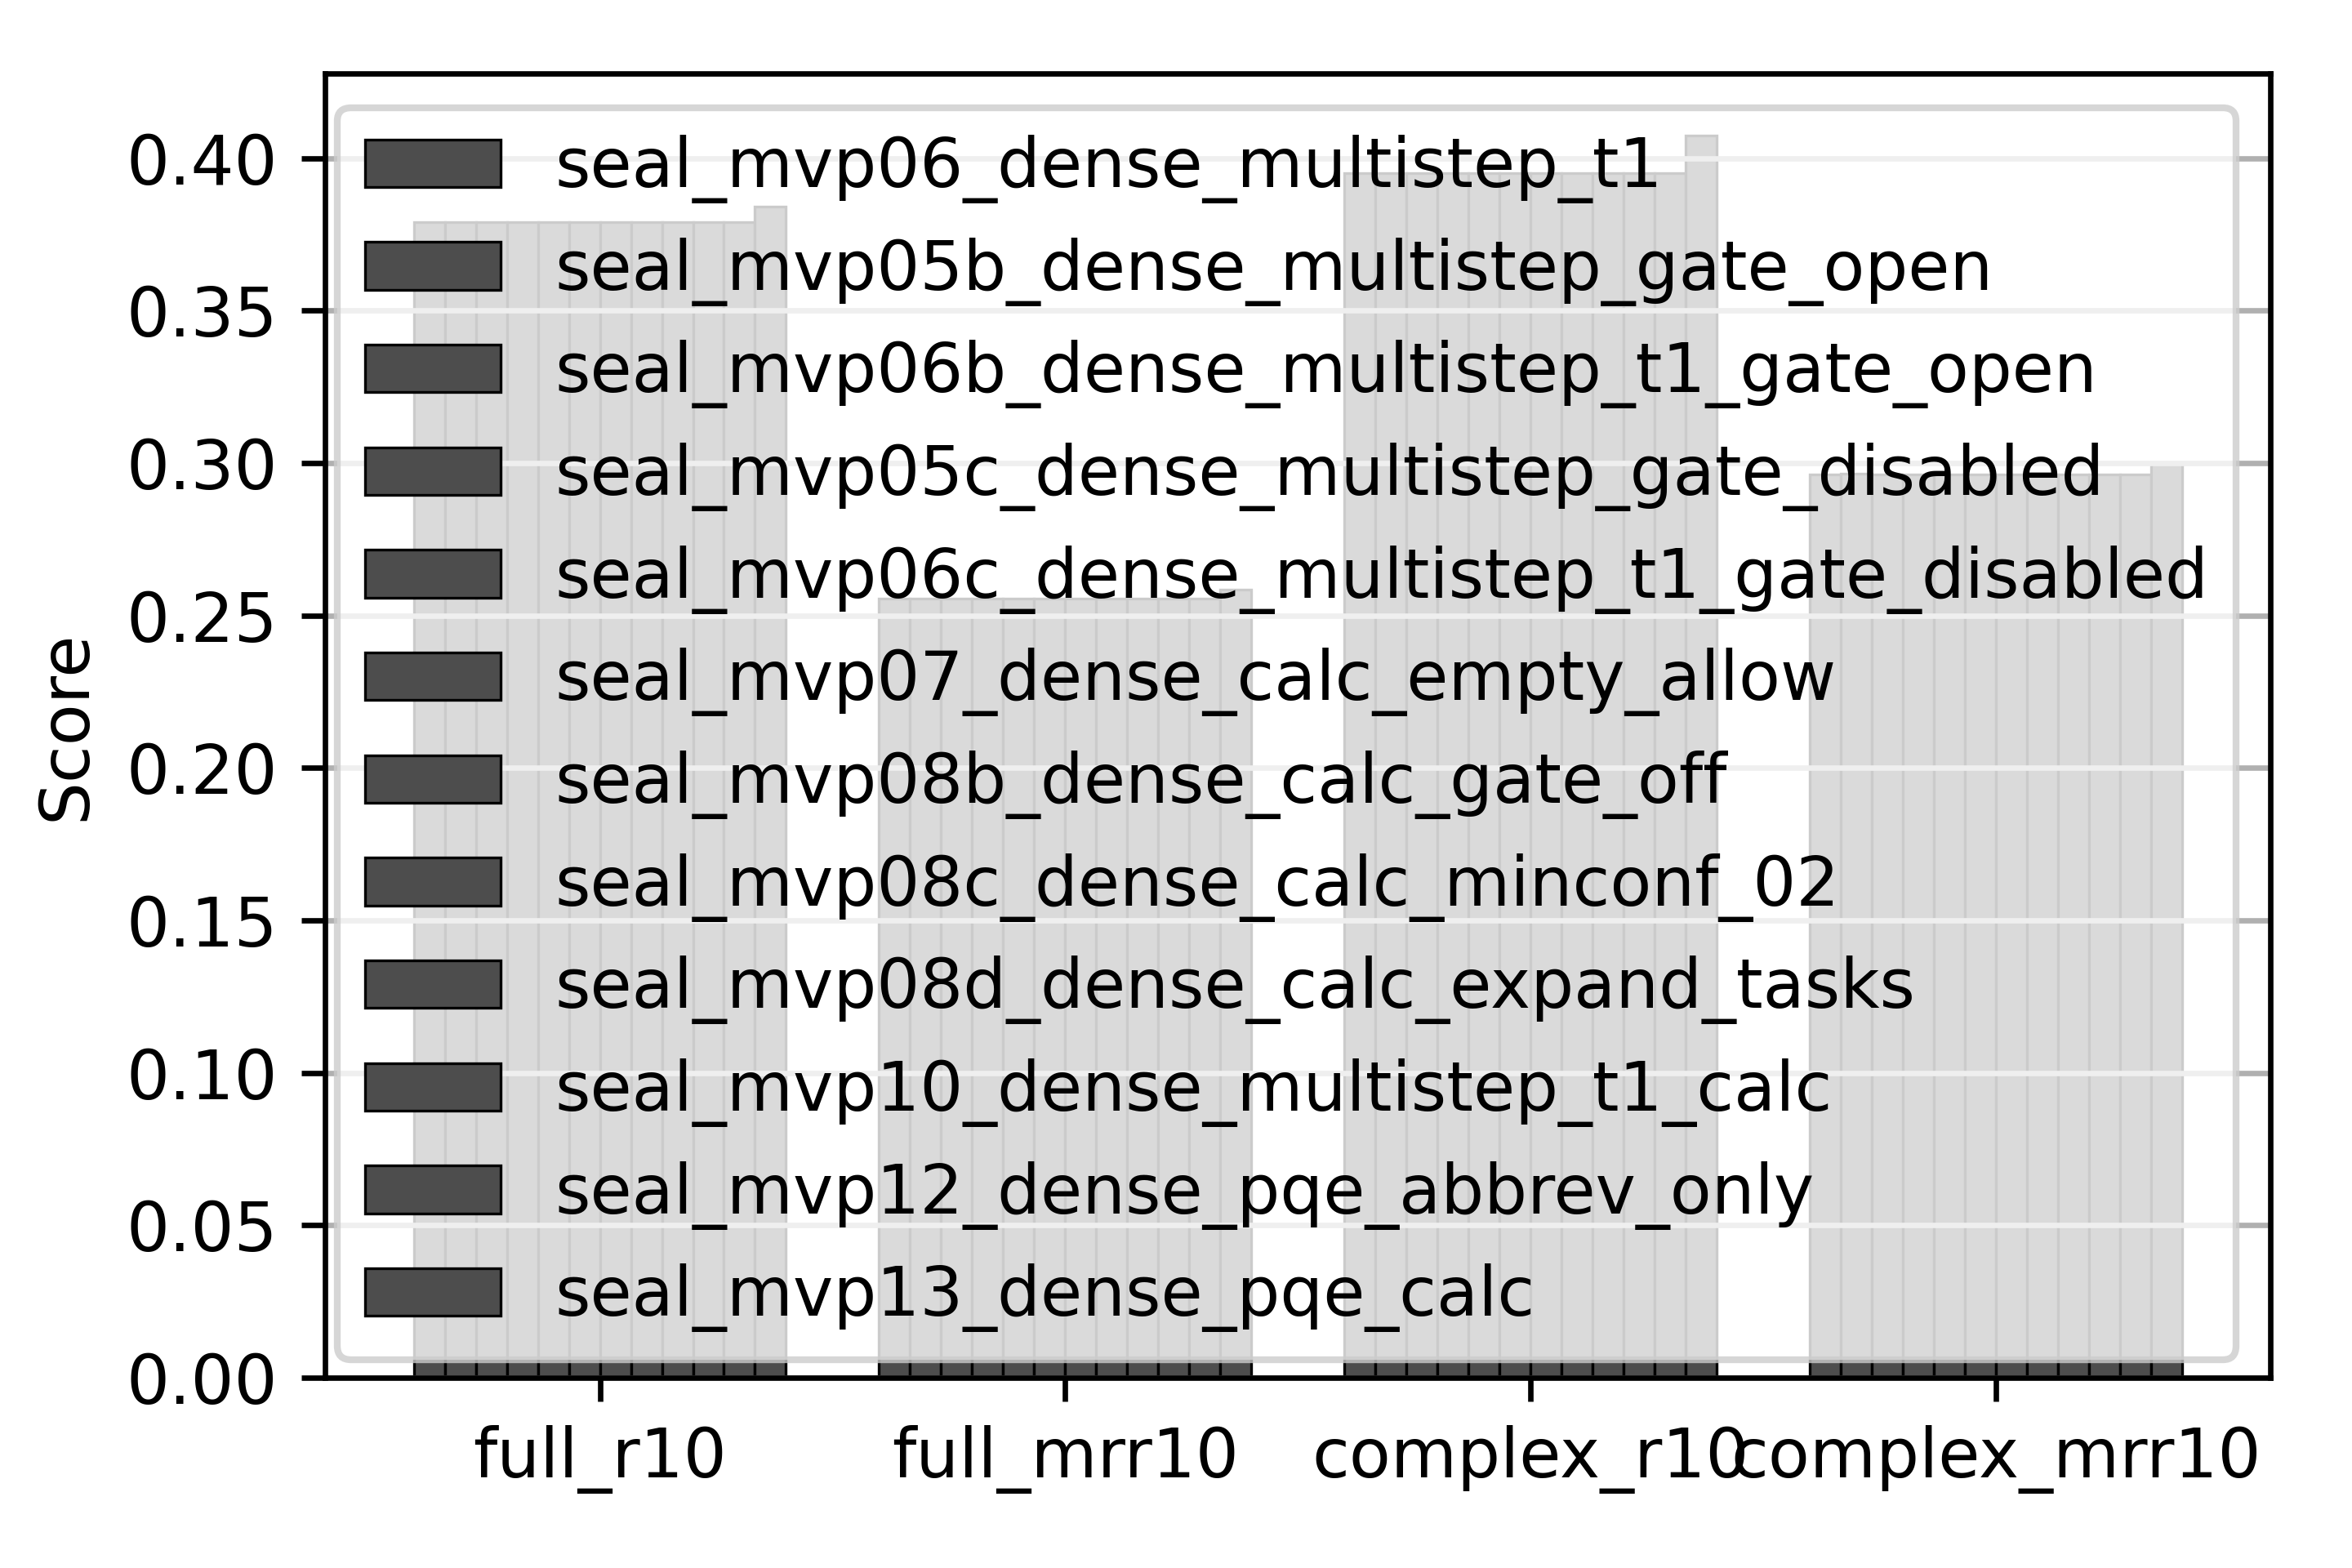
\includegraphics[width=0.9\textwidth]{../thesis/figures_seal/ThemeA/figures/ablation_breakdown.png}
\caption{SEAL 消融拆解图（复用仓库现有图）。\\这张图回答什么问题：基线、增强模块和组合模块之间的增减关系是什么？}
\end{figure}

\textbf{复用现有实验图 2：缩写子集对比}
\begin{figure}[H]
\centering
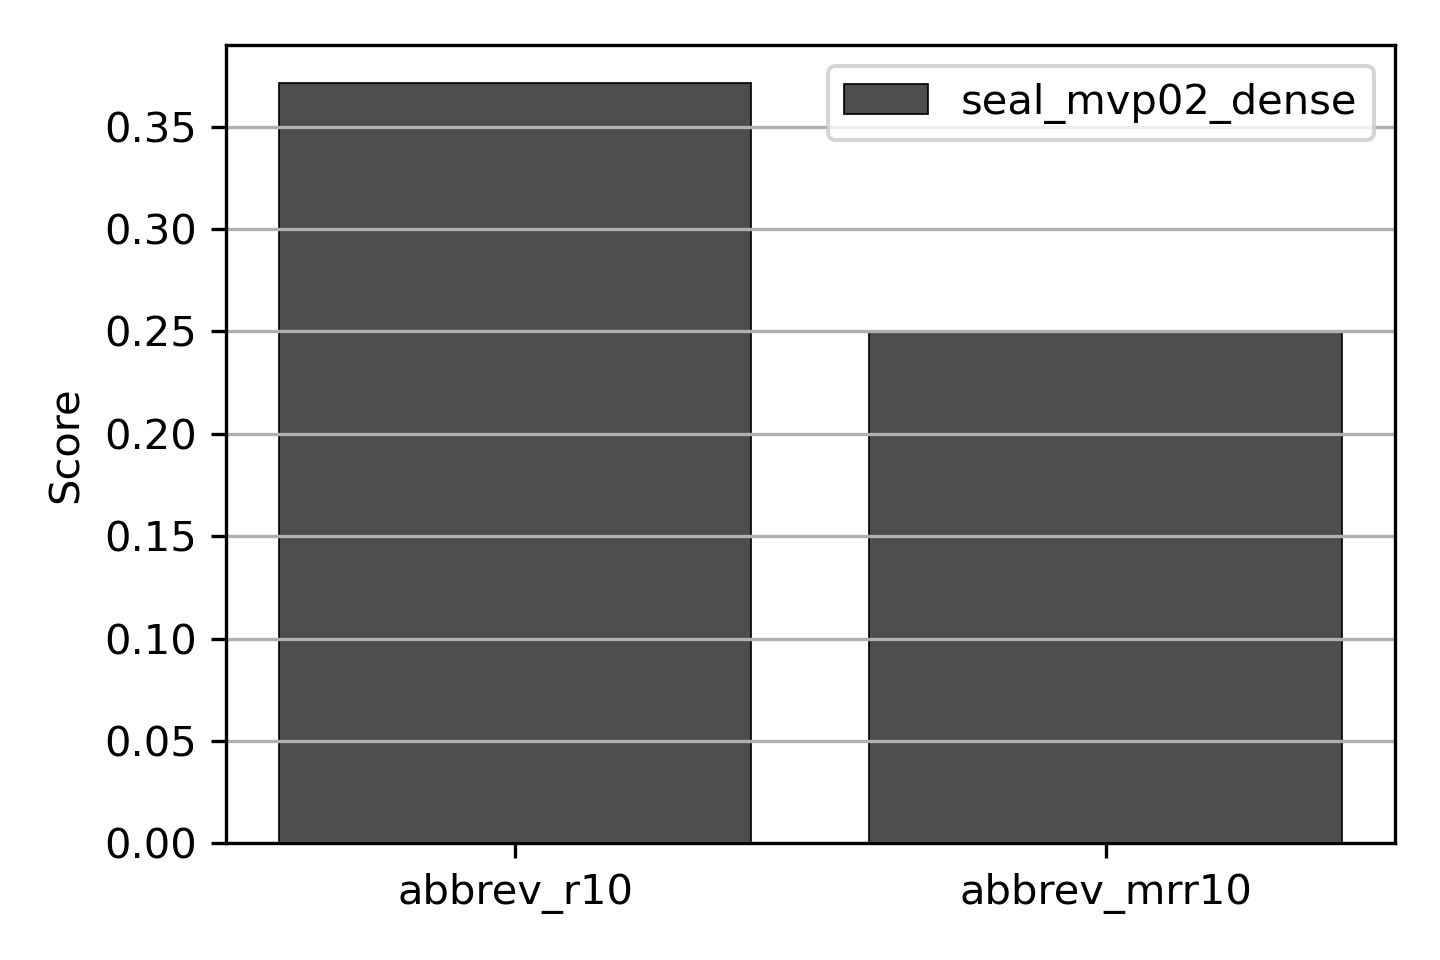
\includegraphics[width=0.88\textwidth]{../thesis/figures_seal/ThemeA/figures/abbrev_breakdown.png}
\caption{缩写子集表现图（复用仓库现有图）。\\这张图回答什么问题：面对缩写密集问题，不同策略在召回与排序上谁更稳？}
\end{figure}

\subsection{易错点}
\begin{itemize}
  \item 只看单个 run，不看成组对照，容易误判模块贡献。
  \item 把 m20 检索侧提升直接当成数值侧闭环，这是跨指标偷换。
  \item 忽略“主 baseline”定义：里程碑将 m12 视为 calculator 主对照，不是 m11。
\end{itemize}

\subsection{自测题}
\begin{enumerate}
  \item 为什么 m19 能作为“PRF-year 有效性”的反事实对照？
  \item m13 相比 m12 告诉我们怎样的门控代价？
  \item m20 的结果为什么属于“弱结论”而不是“强结论”？
\end{enumerate}

\section{关键结论}
\subsection{先讲直觉}
关键结论要满足两个条件：\textbf{指标改善稳定} + \textbf{模块归因清楚}。
只满足其一，都不应该写成主结论。

\subsection{再讲定义}
本讲义采用三层结论框架：
\begin{enumerate}
  \item 强结论：可进摘要与主结论；
  \item 弱结论：有信号但未闭环；
  \item 负结论：在当前口径下未见净增益。
\end{enumerate}

\subsection{再讲本报告中的实现与结果}
\textbf{强结论 1：Retriever FT 是当前最稳增益来源。}
\begin{itemize}
  \item m01$\rightarrow$m02：full\_r10 +0.0543；full\_mrr10 +0.0524。
  \item complex\_r10 +0.0494；abbrev\_r10 +0.0539。
  \item 说明不是局部偶然提升，而是检索底座整体上移。
\end{itemize}

\textbf{强结论 2：Dense 是当前主模式。}
\begin{itemize}
  \item m02 对 m03（BM25）有显著优势；
  \item m04（Hybrid）虽优于 BM25，但仍弱于 m02。
\end{itemize}

\textbf{中等结论：PQE（含年份扩展）可替代 multistep 作为主增益路径。}
\begin{itemize}
  \item m18 比 m02 有一致小幅提升；
  \item m19（abbrev-only）回落到 m02 水平，支持“主增益来自年份相关扩展”。
\end{itemize}

\subsection{易错点}
\begin{itemize}
  \item 把“提升幅度不大”误判为“没有价值”。稳定小幅提升在工程系统中同样重要。
  \item 把“单次高点”当稳定结论。这里强调的是多指标一致、对照清晰。
\end{itemize}

\subsection{自测题}
\begin{enumerate}
  \item 为什么 m01$\rightarrow$m02 可以独立成立为主结论？
  \item PQE 的证据链为什么需要 m19 这种反事实 run？
  \item 强结论与弱结论在证据要求上有什么区别？
\end{enumerate}

\section{负结论与局限}
\subsection{先讲直觉}
负结论不是失败，而是把“看起来合理但当前无效”的路径排除掉。
这会让后续研究更聚焦、更省时间。

\subsection{再讲定义}
\textbf{负结论}：在既定数据与口径下，模块没有产生可观测净增益。  
\textbf{未闭环}：某些指标改善，但未转化为最终质量同步提升。

\subsection{再讲本报告中的实现与结果}
\textbf{负结论 1：multistep 当前未见净增益。}
\begin{itemize}
  \item m05、m07、m09 与 m02 几乎持平。
  \item 结论是“当前实现和口径下无增益”，不是“多步检索理论无效”。
\end{itemize}

\textbf{负结论 2：calculator 出现 coverage-EM 背离。}
\begin{itemize}
  \item m12$\rightarrow$m13：coverage 从 0.6695 到 0.6824，但 EM 从 0.3197 到 0.2867。
  \item m12$\rightarrow$m15：coverage 同样上升，但 EM 仍下降。
\end{itemize}

\textbf{弱结论：组合模块 C（m20）有交互，无闭环。}
\begin{itemize}
  \item 与 m12 比：coverage +0.0172，EM -0.0118。
  \item 说明 retrieval 侧提升确实把更多样本送入 numeric 路由，
  但尚未转化为更高质量数值答案。
\end{itemize}

\textbf{局限披露：子集路径仍需完全对齐。}
里程碑中已提示 \texttt{subsets\_v2} 概念修正存在，但部分 resolved config 仍指向旧路径，
论文写作应明确披露这一点，避免口径误解。

\subsection{易错点}
\begin{itemize}
  \item 把“有交互信号”直接写成“方法有效”。
  \item 把“局限披露”理解为减分。事实上完整披露会提升研究可信度。
\end{itemize}

\subsection{自测题}
\begin{enumerate}
  \item multistep 当前结果应该如何在论文中表述才严谨？
  \item 为什么 m20 不能写成“正向主结论”？
  \item coverage 与 EM 的权衡在系统设计上意味着什么？
\end{enumerate}

\section{复现实操}
\subsection{先讲直觉}
复现不是“把命令跑一遍”，而是确保别人用同一口径能得到同一结论。
因此必须固定事实源、命令顺序和产物边界。

\subsection{再讲定义}
根据仓库封条规则，当前采用 commit-safe 证据面：
\texttt{docs/TABLE\_*.md}、\texttt{docs/SEAL\_*.md}、\texttt{thesis/figures\_seal/**}。  
\texttt{outputs/**} 可用于本地审计，但不作为远端提交边界。

\subsection{再讲本报告中的实现与结果}
\textbf{规范复现顺序（四步）}：
\begin{enumerate}
  \item 先烟雾测试（必须先跑）：
\begin{verbatim}
python scripts/smoke.py --config configs/smoke.yaml --run-id seal_final_smoke
\end{verbatim}
  \item 再跑 seal 矩阵：
\begin{verbatim}
python scripts/run_matrix_step6.py --base-config configs/step6_base.yaml \
  --matrix configs/step6_matrix_seal.yaml
\end{verbatim}
  \item 生成主表：
\begin{verbatim}
python scripts/make_tables.py --experiments configs/step6_experiments_seal.yaml
\end{verbatim}
  \item 生成图表：
\begin{verbatim}
python scripts/plot_all.py --config scripts/plot_config.yaml
\end{verbatim}
\end{enumerate}

\textbf{本讲义自身编译方式（本目录）}：
\begin{verbatim}
powershell -ExecutionPolicy Bypass -File .\build_report_lecture.ps1
\end{verbatim}

\subsection{易错点}
\begin{itemize}
  \item 直接使用旧 matrix 配置，导致表与图和正文口径不一致。
  \item 跳过 smoke，违反工程策略，也增加后续排错成本。
  \item 只留 outputs，不更新 docs/TABLE\_*.md。
\end{itemize}

\subsection{自测题}
\begin{enumerate}
  \item 为什么 smoke 必须在实验前执行？
  \item 为什么论文正文应优先引用 docs/TABLE\_*.md？
  \item “可复现”和“可审计”的区别是什么？
\end{enumerate}

\section{总结与自测}
\subsection{先讲直觉}
这份讲义真正想帮你建立的是一个判断框架：
面对一个模块，不问“新不新”，先问“有没有干净证据证明它有效”。

\subsection{再讲定义}
你当前项目的最稳主线可以压缩为三句话：
\begin{enumerate}
  \item 先把检索底座做好（Retriever FT + Dense 主模式）；
  \item 再做受控扩展（PQE 尤其是年份扩展）；
  \item 数值侧继续聚焦路由质量与闭环，不急于扩大任务空间。
\end{enumerate}

\subsection{再讲本报告中的实现与结果}
\textbf{一句话总评}：  
当前证据清楚支持“检索侧已形成稳定主增益”，
而“数值侧与组合模块 C 仍处于诊断和闭环前阶段”。

\textbf{你下一步最值得投入的方向}：
\begin{itemize}
  \item 对齐并冻结子集路径口径；
  \item 强化 numeric 路由诊断（task dispatch / fact filtering / fallback 质量）；
  \item 在闭环证据出现前，谨慎对外宣称组合模块贡献。
\end{itemize}

\subsection{易错点}
\begin{itemize}
  \item 把“做了很多模块”当“论文贡献完整”。
  \item 为了叙事完整而弱化负结论，反而会损害可信度。
\end{itemize}

\subsection{自测题}
\begin{enumerate}
  \item 如果答辩老师问“你的核心贡献是什么”，你怎么用 30 秒回答？
  \item 如果被追问“为什么多步检索没效果”，你怎么严谨表述？
  \item 如果被追问“m20 是不是成功了”，你怎么解释“有交互但未闭环”？
\end{enumerate}

\appendix
\section{附录：关键指标速查卡}
\begin{longtable}{>{\raggedright\arraybackslash}p{2.6cm} >{\raggedright\arraybackslash}p{10.7cm}}
\toprule
指标/概念 & 快速解释 \\
\midrule
\endhead
R@10 & 前 10 条候选里覆盖正确证据的能力，解决“找没找回来”。 \\
MRR@10 & 正确证据在候选中的前置程度，解决“排得靠不靠前”。 \\
numeric EM & 数值答案在统一精度下是否命中，解决“算得准不准”。 \\
coverage & 是否给出可解析数值答案，解决“答得出来多少”。 \\
强结论 & 多指标一致改善，且可清楚归因到具体模块开关。 \\
弱结论 & 出现局部正信号，但未形成全链路质量闭环。 \\
负结论 & 在当前设置下无净增益，帮助排除无效路径。 \\
\bottomrule
\end{longtable}

\section{附录：证据源定位}
\begin{itemize}
  \item 开题报告：\texttt{报告/开题报告\_石延斌\_U202216405\_题目\_2026年3月11日.pdf}
  \item 主结果：\texttt{docs/TABLE\_MAIN.md}
  \item 数值结果：\texttt{docs/TABLE\_NUMERIC.md}
  \item 里程碑解释：\texttt{docs/MILESTONE\_REPORT.md}
  \item SEAL 状态：\texttt{docs/SEAL\_FINAL\_CHECK.md}
  \item 现有实验图：\texttt{thesis/figures\_seal/ThemeA/figures/ablation\_breakdown.png}、
  \texttt{thesis/figures\_seal/ThemeA/figures/abbrev\_breakdown.png}
\end{itemize}

\section{附录：最小案例推演}
\subsection*{案例 1：缩写密集查询}
\textbf{题型示例}：``比较某公司近两年 EPS 与 EBITDA 的变化。''  
\textbf{推演步骤}：
\begin{enumerate}
  \item 先识别缩写词（EPS、EBITDA）并建立术语映射；
  \item 检索层优先采用 Dense 主模式，再用关键词兜底；
  \item 若原始查询年份信息不足，触发年份感知扩展；
  \item 返回证据时保留来源段落与年份标签，便于核查。
\end{enumerate}
\textbf{你应关注的诊断点}：
\begin{itemize}
  \item 缩写映射是否把术语解释错位；
  \item 检索命中是否落在正确年份段落；
  \item top-k 中正确证据位置是否足够靠前。
\end{itemize}

\subsection*{案例 2：跨年份比较查询}
\textbf{题型示例}：``公司风险因素在 2023 与 2024 年变化最大的条目是什么？''  
\textbf{推演步骤}：
\begin{enumerate}
  \item 原始查询先做种子检索，抽取候选年份线索；
  \item 对年份变体做受控扩展，避免无约束改写；
  \item 用融合分数重排，优先保留双年份都命中的证据；
  \item 输出答案时附上两年对应证据段，避免主观总结。
\end{enumerate}
\textbf{你应关注的诊断点}：
\begin{itemize}
  \item 年份实体是否被错误扩展到不相关年份；
  \item 两个年份证据是否来自同一语义口径；
  \item 系统是否只给结论不提供可核验证据。
\end{itemize}

\subsection*{案例 3：数值计算查询}
\textbf{题型示例}：``请给出某指标同比增速并说明计算依据。''  
\textbf{推演步骤}：
\begin{enumerate}
  \item 先识别任务类型（同比 / 差值 / 比例）；
  \item 抽取操作数、单位、年份并做一致性校验；
  \item 仅在门控通过时调用计算器；
  \item 若门控失败，回退到证据抽取答案并显式说明原因。
\end{enumerate}
\textbf{你应关注的诊断点}：
\begin{itemize}
  \item coverage 上升是否伴随 EM 下降；
  \item 回退路径的答案是否可读且可核对；
  \item 计算触发比例是否过高导致误算扩散。
\end{itemize}

\subsection*{案例 4：组合模块 C 诊断}
\textbf{题型示例}：``在启用 PQE+calculator 后，系统是否整体更好？''  
\textbf{推演步骤}：
\begin{enumerate}
  \item 先看检索侧指标是否提升（m20 相比 m12）；
  \item 再看数值侧是否同步提升（EM 与 coverage）；
  \item 若仅 coverage 提升，判定为有交互但未闭环；
  \item 将结果归入弱结论，不上升为主贡献。
\end{enumerate}
\textbf{你应关注的诊断点}：
\begin{itemize}
  \item 是否发生跨指标偷换（检索增益替代数值闭环）；
  \item 是否存在只强调可回答率、不强调准确率的偏差；
  \item 结论是否与里程碑分层口径一致。
\end{itemize}

\section{附录：答辩口径与自查清单}
\subsection*{高频追问的标准回答框架}
\begin{longtable}{>{\raggedright\arraybackslash}p{3.0cm} >{\raggedright\arraybackslash}p{10.3cm}}
\toprule
可能问题 & 建议回答框架 \\
\midrule
\endhead
你的核心贡献是什么？ & 先给一句话主结论：检索侧形成稳定增益；再给两组证据：m01$\rightarrow$m02、m02$\rightarrow$m18；最后明确边界：数值侧未闭环。 \\
为什么多步检索没有提升？ & 强调“当前实现和口径下无净增益”，并给 m05/m07/m09 与 m02 基本持平的证据；不把它扩大为理论无效。 \\
为什么不直接强调组合模块 C？ & 给出 m20 与 m12 的 numeric 对比：coverage 上升但 EM 下降；说明其定位是弱结论与后续工作入口。 \\
你的工作可复现吗？ & 说明 canonical 四步命令、SEAL matrix 全部 ok、主表与图均可重建；并区分 commit-safe 证据面与本地审计产物。 \\
你和已有 RAG 工作的区别？ & 不是只做通用 RAG，而是围绕金融场景的年份对齐与数值可靠性，做模块化协同与可归因消融。 \\
\bottomrule
\end{longtable}

\subsection*{提交前 15 条自查清单}
\begin{enumerate}
  \item 所有关键数字与 \texttt{TABLE\_MAIN/TABLE\_NUMERIC} 完全一致。
  \item 强/弱/负结论分层与 \texttt{MILESTONE\_REPORT.md} 一致。
  \item 没有把 coverage 提升写成闭环成功。
  \item 没有把局部信号写成全局主结论。
  \item 所有图都写清楚“这张图回答什么问题”。
  \item 公式后面都有“公式含义 + 一句话例子”。
  \item 每章都有易错点与自测题。
  \item 复现部分明确 smoke 在先。
  \item 复现部分区分 commit-safe 与 outputs 审计层。
  \item 对 multistep 的表述是“当前无净增益”，不是“理论无效”。
  \item 对组合模块 C 的表述是“有交互、未闭环”。
  \item 子集口径风险被明确披露，不回避。
  \item 所有路径名、run 名字可在仓库中对应到实际文件。
  \item 讲义语言以中文为主，英文缩写都给了中文语境解释。
  \item 最终 PDF 编译通过且无缺图。
\end{enumerate}

\end{document}
